% Options for packages loaded elsewhere
\PassOptionsToPackage{unicode}{hyperref}
\PassOptionsToPackage{hyphens}{url}
%
\documentclass[
  12pt,
]{article}
\title{Blue Mesa Power Production Analysis}
\usepackage{etoolbox}
\makeatletter
\providecommand{\subtitle}[1]{% add subtitle to \maketitle
  \apptocmd{\@title}{\par {\large #1 \par}}{}{}
}
\makeatother
\subtitle{Web address for GitHub repository}
\author{Stephanie Kinser, Katie Owens, Cassidy White}
\date{}

\usepackage{amsmath,amssymb}
\usepackage{lmodern}
\usepackage{iftex}
\ifPDFTeX
  \usepackage[T1]{fontenc}
  \usepackage[utf8]{inputenc}
  \usepackage{textcomp} % provide euro and other symbols
\else % if luatex or xetex
  \usepackage{unicode-math}
  \defaultfontfeatures{Scale=MatchLowercase}
  \defaultfontfeatures[\rmfamily]{Ligatures=TeX,Scale=1}
  \setmainfont[]{Times New Roman}
\fi
% Use upquote if available, for straight quotes in verbatim environments
\IfFileExists{upquote.sty}{\usepackage{upquote}}{}
\IfFileExists{microtype.sty}{% use microtype if available
  \usepackage[]{microtype}
  \UseMicrotypeSet[protrusion]{basicmath} % disable protrusion for tt fonts
}{}
\makeatletter
\@ifundefined{KOMAClassName}{% if non-KOMA class
  \IfFileExists{parskip.sty}{%
    \usepackage{parskip}
  }{% else
    \setlength{\parindent}{0pt}
    \setlength{\parskip}{6pt plus 2pt minus 1pt}}
}{% if KOMA class
  \KOMAoptions{parskip=half}}
\makeatother
\usepackage{xcolor}
\IfFileExists{xurl.sty}{\usepackage{xurl}}{} % add URL line breaks if available
\IfFileExists{bookmark.sty}{\usepackage{bookmark}}{\usepackage{hyperref}}
\hypersetup{
  pdftitle={Blue Mesa Power Production Analysis},
  pdfauthor={Stephanie Kinser, Katie Owens, Cassidy White},
  hidelinks,
  pdfcreator={LaTeX via pandoc}}
\urlstyle{same} % disable monospaced font for URLs
\usepackage[margin=2.54cm]{geometry}
\usepackage{graphicx}
\makeatletter
\def\maxwidth{\ifdim\Gin@nat@width>\linewidth\linewidth\else\Gin@nat@width\fi}
\def\maxheight{\ifdim\Gin@nat@height>\textheight\textheight\else\Gin@nat@height\fi}
\makeatother
% Scale images if necessary, so that they will not overflow the page
% margins by default, and it is still possible to overwrite the defaults
% using explicit options in \includegraphics[width, height, ...]{}
\setkeys{Gin}{width=\maxwidth,height=\maxheight,keepaspectratio}
% Set default figure placement to htbp
\makeatletter
\def\fps@figure{htbp}
\makeatother
\setlength{\emergencystretch}{3em} % prevent overfull lines
\providecommand{\tightlist}{%
  \setlength{\itemsep}{0pt}\setlength{\parskip}{0pt}}
\setcounter{secnumdepth}{5}
\usepackage{amsmath}
\usepackage{booktabs}
\usepackage{caption}
\usepackage{longtable}
\ifLuaTeX
  \usepackage{selnolig}  % disable illegal ligatures
\fi

\begin{document}
\maketitle

\newpage
\tableofcontents 
\newpage
\listoftables 
\newpage
\listoffigures 
\newpage

\hypertarget{rationale-and-research-questions}{%
\section{Rationale and Research
Questions}\label{rationale-and-research-questions}}

Climate patterns have a significant impact on business, health, and
community well-being. The western United States has been experiencing
years of low precipitation and prolonged drought. Currently, all of
Colorado is experiencing a moderate to extreme drought (Drought.gov).
The National Oceanic and Atmospheric Administration's (NOAA) National
Integrated Drought Information System (NIDIS) tracks the impacts of
drought, including its effect on crops and livestock and fire. We want
to explore the effects of climate patterns on hydroelectric power
production, an impact that is not currently captured by NIDIS.

Hydroelectric power plants rely on a sufficient reservoir level to
maintain power output, which can be an important source of carbon-free
electricity. We wonder how climate patterns and reservoir management
have impacted hydroelectric power production. We identified Blue Mesa
Reservoir and Hydroelectric Power Plant in Colorado to explore our
research questions.

Blue Mesa Power Plant has a nameplate capacity of 86.2 MW and began
generating power in 1967. It is located on the Gunnison River in
Colorado.

Research Questions: * Which climate and reservoir management variables
influence Blue Mesa's power production? * How has electricity generation
of Blue Mesa Power Plant changed over time?

\newpage

\hypertarget{dataset-information}{%
\section{Dataset Information}\label{dataset-information}}

For our analysis, we relied on two data sets. For Blue Mesa's power
production and reservoir management, we sourced data from the Colorado
Bureau of Reclamation. The power production dataset includes monthly
electricity generation reported in MWh. The reservoir management dataset
includes eight variables, including elevation, storage, inflow, and
outflow. We pulled monthly averages for this data from 2003 to 2021 when
all the data was available.

We sourced climate data from the Colorado Climate Center, an institute
at Colorado State University. We pulled monthly data for Blue Mesa on
the maximum temperature, minimum temperature, average precipitation, and
average snowfall.

\newpage

\hypertarget{exploratory-analysis}{%
\section{Exploratory Analysis}\label{exploratory-analysis}}

Prior to analysis, data were explored in terms of both summary
statistics and visual patterns and relationships. Table 1 summarizes the
data for all fourteen variables used in building the explanatory model.
Summary statistics include mean, minimum value, maximum value, and
standard deviation across all observations. From 2003 to 2021, Blue Mesa
Reservoir's elevation ranged from 7,438 ft to 7,519 ft. Temperature at
the reservoir ranged from -11.80 \(^\circ\)F to 87.20 \(^\circ\)F. The
Blue Mesa dam produced an average of 18,856 MWh of electricity per month
with a range of 2,724 MWh to 54,068 MWh during peak production.

\captionsetup[table]{labelformat=empty,skip=1pt}
\begin{longtable}{crrrr}
\toprule
Variable & Mean & Min. & Max. & sd \\ 
\midrule
 Elevation.ft & $7,486.00$ & $7,438.00$ & $7,519.00$ & $18.51$ \\ 
  Storage.af & $557,251.00$ & $247,684.00$ & $826,302.00$ & $134,507.54$ \\ 
Evaporation.af & $648.60$ & $114.00$ & $1,544.00$ & $443.68$ \\ 
  Inflow.cfs & $1,139.70$ & $258.00$ & $7,456.00$ & $1,278.05$ \\ 
UnregInflow.cfs & $1,137.00$ & $195.00$ & $7,915.00$ & $1,366.55$ \\ 
  Power.cfs & $1,078.20$ & $186.00$ & $3,118.00$ & $588.99$ \\ 
  Bypass.cfs & $58.88$ & $0.00$ & $2,379.00$ & $252.86$ \\ 
 Spillway.cfs & $-11,550,000.00$ & $-2,147,000,000.00$ & $1,257.00$ & $157,461,141.48$ \\ 
  Total.cfs & $1,146.30$ & $186.00$ & $5,939.00$ & $761.36$ \\ 
     MaxT & $55.13$ & $13.40$ & $87.20$ & $20.75$ \\ 
     MinT & $23.63$ & $-11.80$ & $50.80$ & $16.76$ \\ 
    Precip & $0.73$ & $0.00$ & $4.39$ & $0.61$ \\ 
     Snow & $3.91$ & $0.00$ & $32.90$ & $5.86$ \\ 
     MWH & $18,856.00$ & $2,724.00$ & $54,068.00$ & $10,896.96$ \\ 
\bottomrule
\end{longtable}

To further explore the data, a series of graphs were developed to
visually examine trends in key variables over time and well as variables
with expected trends in relation to each other. In figure 1, both
minimum and maximum temperatures are shown from 2003 until 2021 at Blue
Mesa Reservoir. To examine trends in electricity generation over time,
figure 2 plots MWh production by date (month). In the next plot, figure
3, reservoir elevation (ft) is graphed over time followed by figure 4
showing volume in acre-feet over time. Total inflow over time is then
shown in figure 5.

\begin{figure}

{\centering 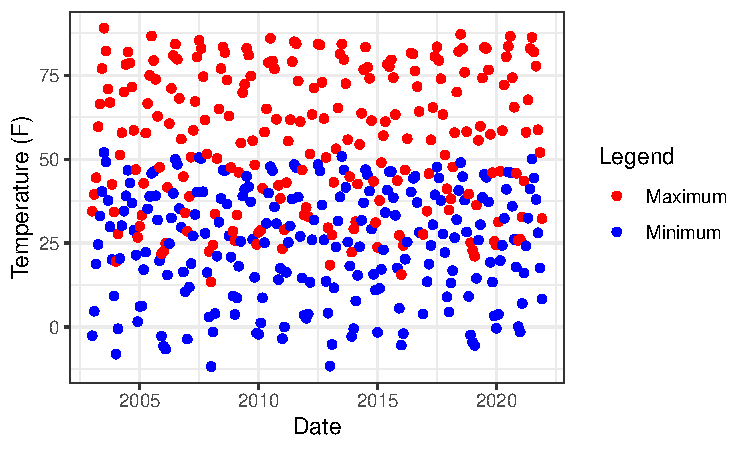
\includegraphics{Project_Report_files/figure-latex/min/max-1} 

}

\caption{Minimum and maximum temperature at Blue Mesa Reservoir in Fahrenheit from January 2003 until December 2021.}\label{fig:min/max}
\end{figure}

\begin{figure}

{\centering 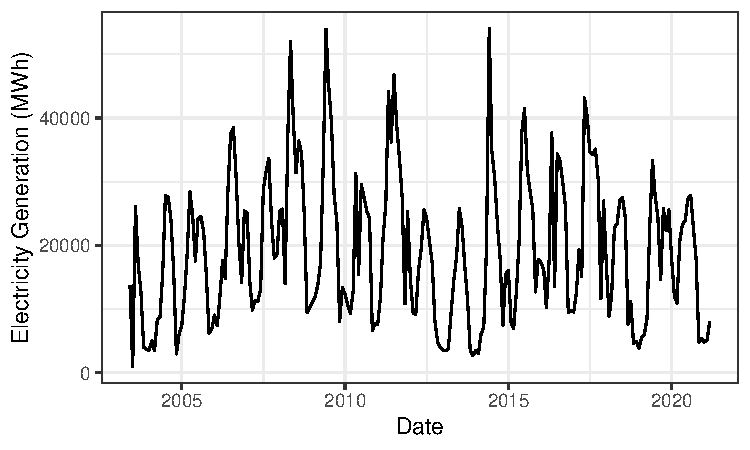
\includegraphics{Project_Report_files/figure-latex/power production-1} 

}

\caption{Power production in megawatt hours at Blue Mesa Reservoir from June 2003 until March 2021.}\label{fig:power production}
\end{figure}

\begin{figure}

{\centering 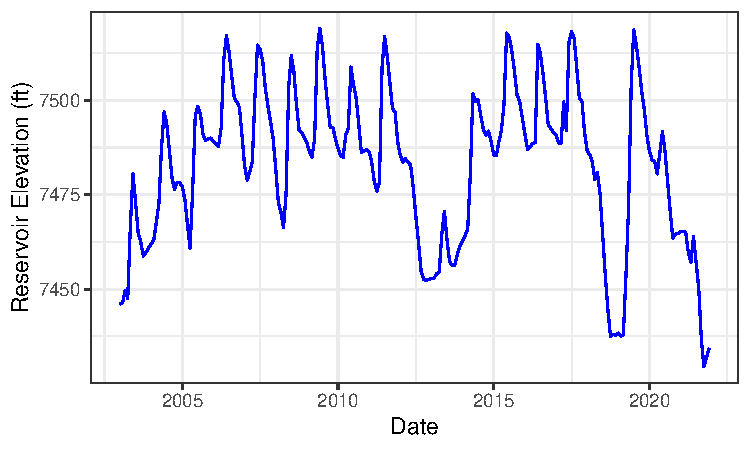
\includegraphics{Project_Report_files/figure-latex/elevation-1} 

}

\caption{Reservoir elevation in feet at Blue Mesa Reservoir from January 2003 until December 2021.}\label{fig:elevation}
\end{figure}

\begin{figure}

{\centering 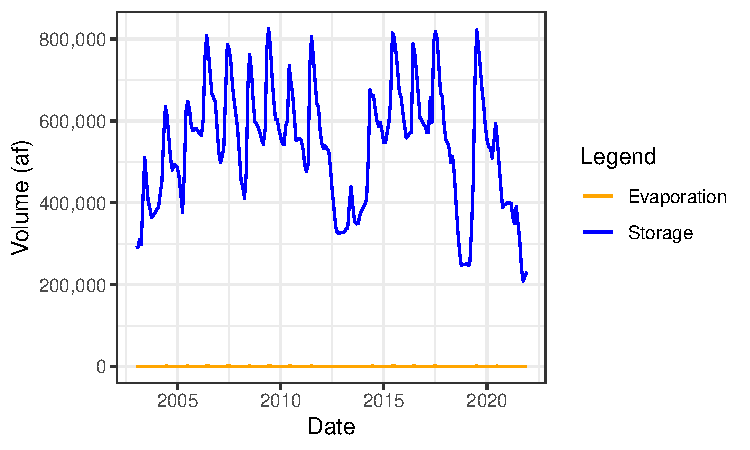
\includegraphics{Project_Report_files/figure-latex/volume-1} 

}

\caption{Reservoir volume in acre-feet at Blue Mesa Reservoir from January 2003 until December 2021.}\label{fig:volume}
\end{figure}

\begin{figure}

{\centering 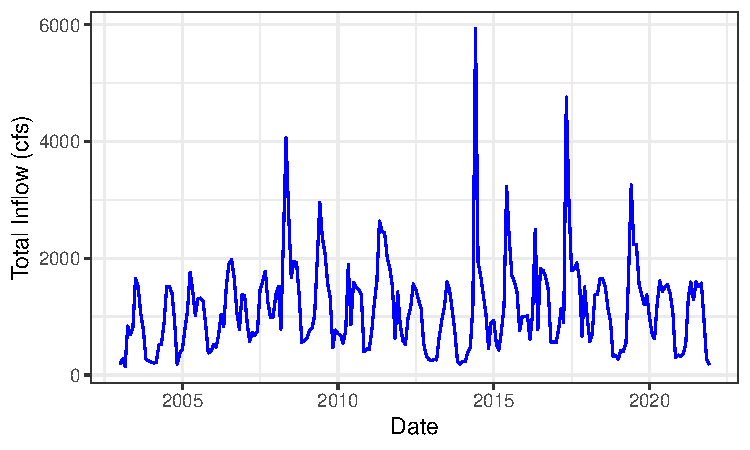
\includegraphics{Project_Report_files/figure-latex/total flow-1} 

}

\caption{Total flow into Blue Mesa Reservoir in cubic feet per second from January 2003 until December 2021.}\label{fig:total flow}
\end{figure}

From there, a few variables are explored graphically with respect to the
dependent variable (MWh). In figure 7, total inflow (cfs) is plotted
against electricity generation and shows a positive relationship. As
inflow increases, electricity generation increases as well.

\begin{figure}

{\centering 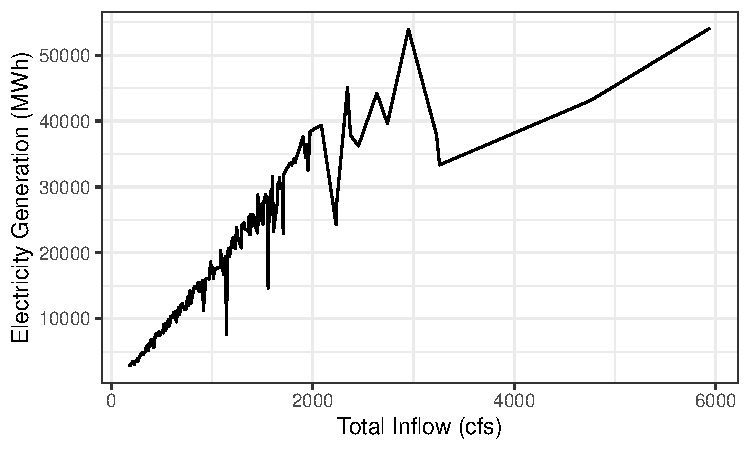
\includegraphics{Project_Report_files/figure-latex/MWHxTotal-1} 

}

\caption{Relationship between total water inflow (cfs) and power production (MWH) at Blue Mesa Reservoir from 2003 until 2021.}\label{fig:MWHxTotal}
\end{figure}

Power outflow is then plotted against electricity generation in figure
8, also showing a positive relationship. These trends were expected
based on the high correlation between total inflow and MWh and power
outflow and MWh as shown in figure 9. However, the relationships between
these variables are explored further in the analysis for significance.

\begin{figure}

{\centering 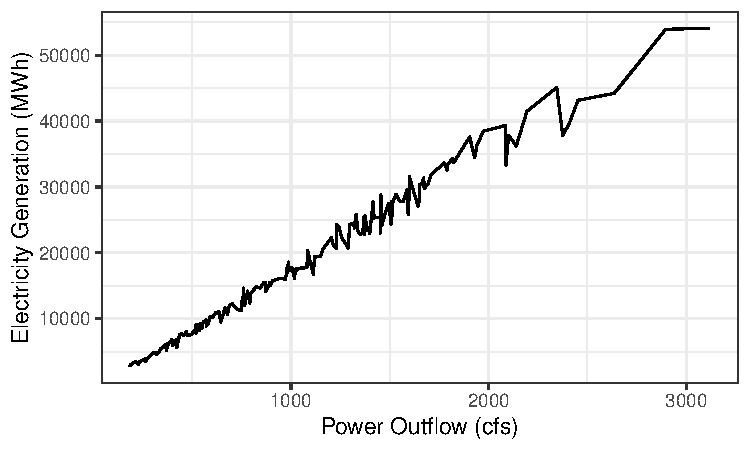
\includegraphics{Project_Report_files/figure-latex/MWHxPower-1} 

}

\caption{Relationship between power outflow (cfs) and power production (MWH) at Blue Mesa Reservoir from 2003 until 2021.}\label{fig:MWHxPower}
\end{figure}

Last, figure 10 shows precipitation (inches) plotted against electricity
generation. No noticeable trend is observed but the contribution from
precipitation in explaining variation in electricity generation is
explored further in the analysis.

\begin{figure}

{\centering 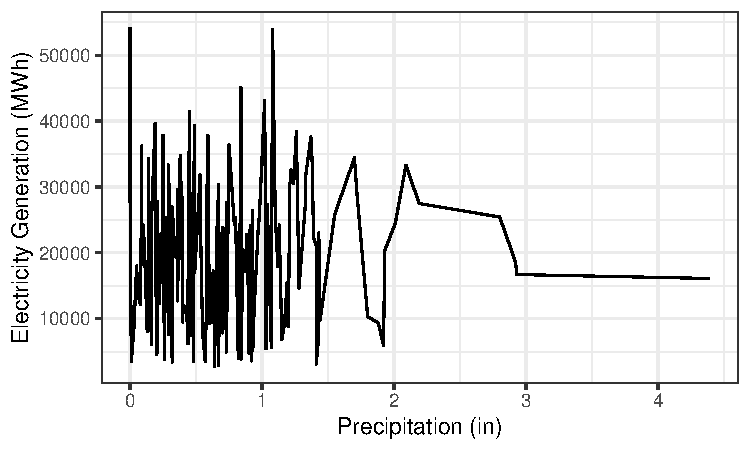
\includegraphics{Project_Report_files/figure-latex/MWHxPrecip-1} 

}

\caption{Relationship between precipitation (inches) and power production (MWH) at Blue Mesa Reservoir from 2003 until 2021.}\label{fig:MWHxPrecip}
\end{figure}

\newpage

\hypertarget{analysis}{%
\section{Analysis}\label{analysis}}

The analysis was divided into two components: a linear regression to
explore the influene of other variables on electricity generation, and a
time series analysis to explore how electricity generation has changed
over time.

\hypertarget{question-1-which-climate-and-reservoir-management-variables-influence-blue-mesas-power-production}{%
\subsection{Question 1: Which climate and reservoir management variables
influence Blue Mesa's power
production?}\label{question-1-which-climate-and-reservoir-management-variables-influence-blue-mesas-power-production}}

The first step in the analysis was to explore the correlation between
different varaibles used in the model. In (figure 9), narrow ovals or
straight lines indicate two variables that are highly correlated. The
wider the oval, the less correlated the variables are. This correlation
matrix provides an understanding of how variables relate to one another
and is useful when interpretting results.

\begin{figure}

{\centering 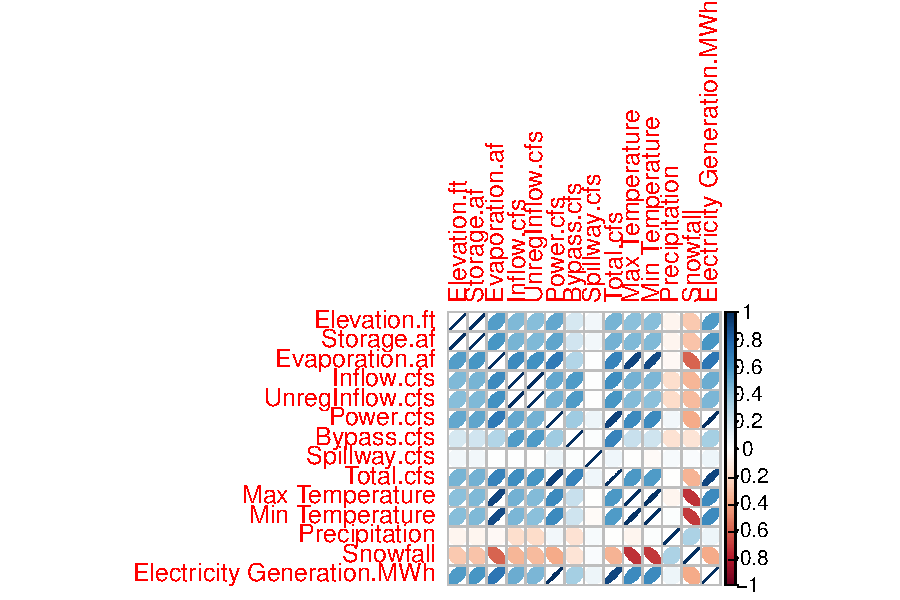
\includegraphics{Project_Report_files/figure-latex/correlation-1} 

}

\caption{Correlation matrix for all dependent and independent variables used in building the explanatory model.}\label{fig:correlation}
\end{figure}

A multiple linear regression was then performed to explore the
contribution of the thirteen independent variables in explaining
variation in the dependent variable, megawatt hours (MWh). After the
initial regression, an AIC test was run to identify which combination of
variables contributed to the model of best fit for explaining MWh. Eight
independent variables were selected for the final model and their
coefficients (Beta) and significance values are summarized in Table 2.

\captionsetup[table]{labelformat=empty,skip=1pt}
\setlength{\LTpost}{0mm}
\begin{longtable}{lccc}
\toprule
\textbf{Characteristic} & \textbf{Beta} & \textbf{95\% CI}\textsuperscript{1} & \textbf{p-value} \\ 
\midrule
Elevation.ft & -249 & -322, -175 & <0.001 \\ 
Storage.af & 0.04 & 0.03, 0.05 & <0.001 \\ 
Evaporation.af & 1.4 & 0.54, 2.2 & 0.001 \\ 
Inflow.cfs & -0.68 & -0.82, -0.55 & <0.001 \\ 
MaxT & -18 & -32, -4.1 & 0.011 \\ 
Precip & 166 & -17, 349 & 0.075 \\ 
Total.cfs & 0.38 & -0.04, 0.80 & 0.075 \\ 
Power.cfs & 17 & 17, 18 & <0.001 \\ 
\bottomrule
\end{longtable}
\begin{minipage}{\linewidth}
\textsuperscript{1}CI = Confidence Interval\\
Adjusted R squared = 1.00; AIC = 2,994\\
\end{minipage}

The final regression identifies elevation, storage, evaporation, inflow,
maximum temperature, precipitation, total inflow, and power outflow as
all contributing to explaining variation in electricity generation (MWh)
across the study period. The model has an adjusted R\^{}2 of 0.995,
indicating the model explains 99.5\% of the variation in MWh. According
to the model results, a decrease in elevation of 249 ft per month leads
to an increase of one MWh of electricity generation. This result is
expected considering that as water is drawn down through the
hydroelectric turbines for electricity generation, the reservoir's
elevation decreases. Likewise, as power outflow increases 17 cfs,
electricity generation increases by one MWh per month. This result also
agrees with our expected findings since power outflow and MWh are highly
correlated and since power outflow is released with the intention of
generating electricity.

\hypertarget{question-2-how-has-electricity-generation-of-blue-mesa-power-plant-changed-over-time}{%
\subsection{Question 2: How has electricity generation of Blue Mesa
Power Plant changed over
time?}\label{question-2-how-has-electricity-generation-of-blue-mesa-power-plant-changed-over-time}}

\newpage

\hypertarget{summary-and-conclusions}{%
\section{Summary and Conclusions}\label{summary-and-conclusions}}

\newpage

\hypertarget{references}{%
\section{References}\label{references}}

\textless add references here if relevant, otherwise delete this
section\textgreater{}

\end{document}
